\documentclass[11pt]{report}

\usepackage[margin=1in]{geometry}
\usepackage{amsmath, amssymb, enumitem, indentfirst, graphicx, float, comment, algorithm2e,listings,xcolor}
\usepackage[style=numeric]{biblatex}
\graphicspath{ {images/} }

\addbibresource{sources.bib}

\setlength{\parindent}{2em}
\setlength{\parskip}{1em}

\title{CS488: Documentation \\ \small{Title:  Jumper}}
\date{\today}
\author{Name: Ramanpreet Nara \\ Student ID: \texttt{20517713} \\ User ID: \texttt{rsnara}}

% set the default code style
\lstset{
    frame=tb, % draw a frame at the top and bottom of the code block
    tabsize=2, % tab space width
    showstringspaces=false, % don't mark spaces in strings
    numbers=left, % display line numbers on the left
    commentstyle=\color{green}, % comment color
    keywordstyle=\color{blue}, % keyword color
    stringstyle=\color{red}, % string color
    language = C++,
    xleftmargin = 2cm,
    xrightmargin = 2cm,
    framexleftmargin = 1em,
    basicstyle=\tiny,
    aboveskip=20pt,
    belowskip=20pt
}

\begin{document}
\maketitle
\tableofcontents
\listoffigures

\lstlistoflistings

\chapter{Introduction}
\section{Purpose}
\begin{enumerate}
\item To build a fun, simple, playable, and hopefully addictive game.
\item To experiment with, and gain a deeper understanding of 3d Graphics, and the OpenGL rendering pipeline. Mainly, I wanted to learn how to: build animations with key-frames, map textures to objects, create 3d scenes, and implement shadows.
\item To gain an understanding of how to architect an OpenGL game.
\end{enumerate}
\section{Statement}
\subsection{Overview}
For this project, I built a simple game using OpenGL. The game consists of multiple levels, each of which is serialized in a JSON file. At each level, the player starts off on a floating platform positioned somewhere in the sky. His objective is to jump from one platform to the next, with the goal of eventually reaching the end without falling off. The more platforms the player visits, the higher his score. When the player falls down, the level and his score reset. When the player reaches the last platform of the current level, he advances to the next level, if one exists. In total, there are three levels.

\subsection{Platforms}
The platforms move sinusoidally in the $x$ direction. Each platform has a timer called $TTL$. When the player first lands on a platform, its $TTL$ starts to decrease. After the player jumps off, the platform's $TTL$ stops decreasing. If a platform's $TTL$ reaches 0, the platform begins to experience gravitational and wind forces, which makes the platform fall. If the player is standing on the falling platform, the player falls along with the platform. This incentivizes the player to be quick on his feet in moving from one platform to the next.

\begin{figure}[H]
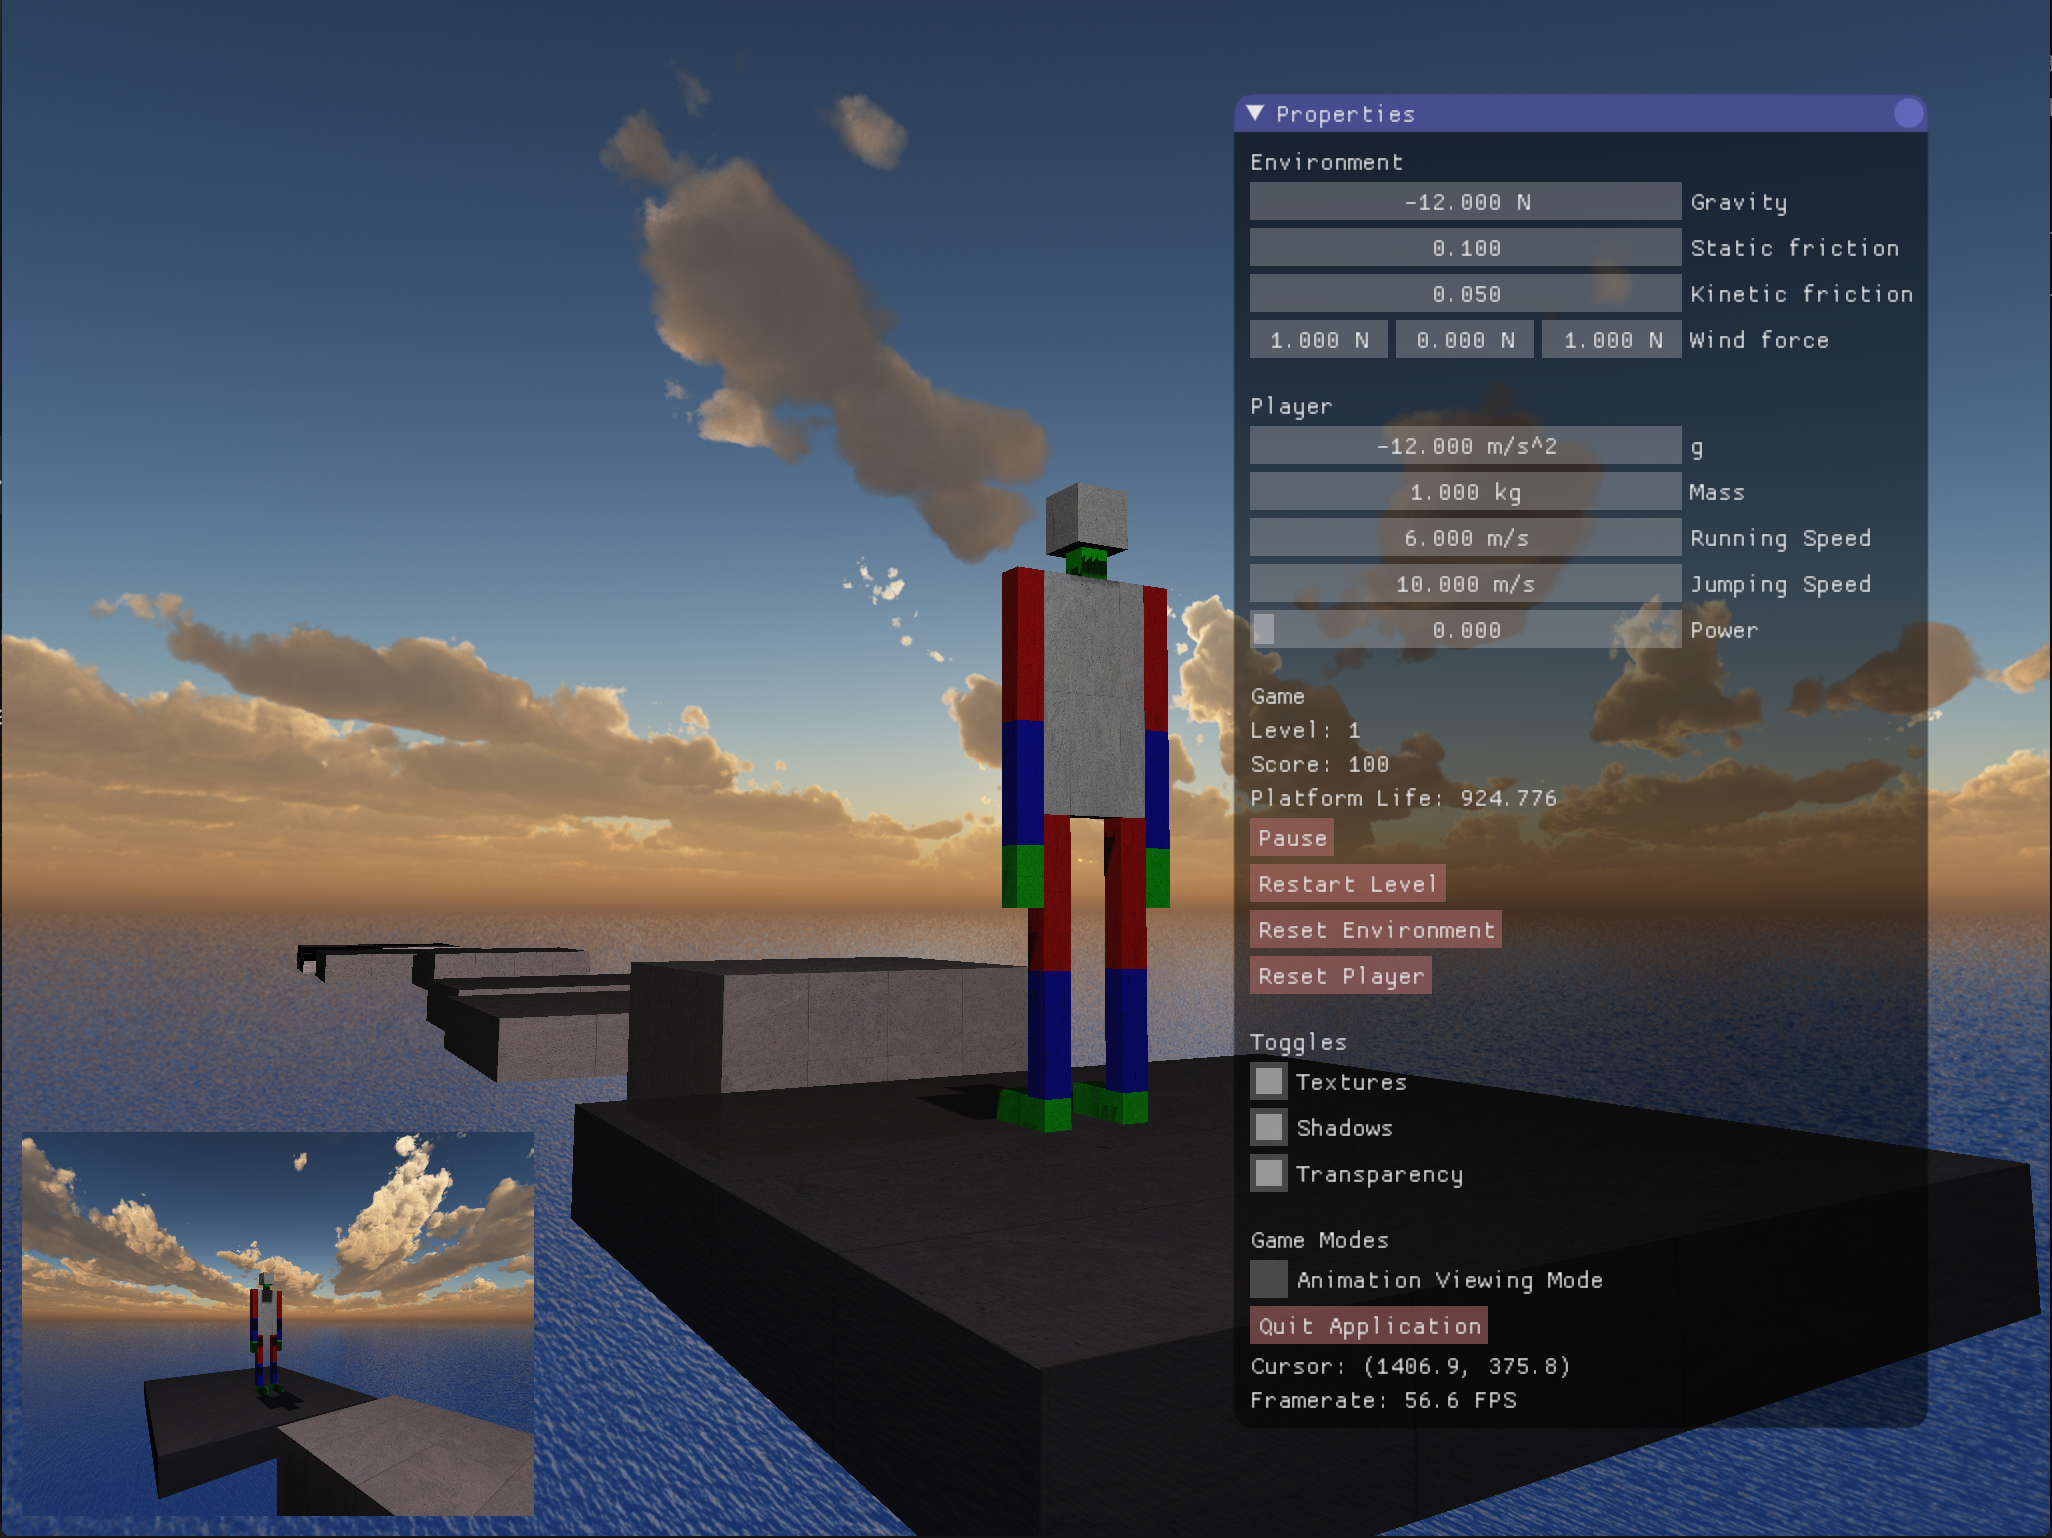
\includegraphics[width=8cm]{start.png}
\centering
\caption{The player standing on the starting platform in Level 1.}
\end{figure}

\subsection{Levels}
Since each level is deserialized from a JSON file when the game starts, players can build and play their own levels. This ultimately increases the playability the game. This setup also makes it easier to develop and test levels, which helped me iterate quickly on the gameplay mechanics while I was developing the game.

\subsection{Executing plan of attack}
% Restructure
For this project, I animated the puppet I created in Assignment 3. First, I gave him the ability to run, and jump. This required me to implement a very basic physics engine to simulate gravity. Lua was used to create the scene node hierarchy that rendered the puppet on to the screen. The actual rendering involved implementing the Visitor design pattern. This pattern was used to traverse the scene node hierarchy, collect the joint transformations, and render the geometry nodes in their correct locations and orientations.

After the puppet was implemented, he was animated using keyframe animation. This involved specifying the joint angles of the puppet for each keyframe. Each keyframe was then associated with a time. Then, whenever the puppet was rendered, I found the keyframes that temporally surrounded the current time. Using this keyframe pair and the current time, I interpolated the set of joint angles for the puppet at the current time. This set was passed to the rendering visitor, which rendered the puppet in various stages of animation.

After animations were completed, the physics engine was extended to support wind force, and friction. Then, collisions were added. This allowed the puppet to fall down from platforms and added a bit of realism to his in-game movements.

After finishing up the collisions, shadows were implemented using a technique called shadow mapping. This technique is discussed with great detail in later sections of the report.

After shadows were implemented, transparency was implemented by turning on back-face culling, sorting the objects with respect to their proximity to the camera, and rendering them in reverse order. The alpha channel was used to make objects transparent.

OpenAL was used to implement synchronized sound. Sound synchronization was achieved was by associating a keyframe with a sound buffer. Then, whenever the current frame moved into a new keyframe pair $[k_1, k_2]$, the sound associated with $k_1$, if any, would be played.

Finally, texture mapping was implemented by generating meshes containing UV coordinates with Blender. Then, \verb|MeshConsolidator| was modified to read in these meshes. The UV data was then bound to its own Vertex Buffer Object and fead in as inputs to the Vertex shader. The vertex shader forwarded this data to the fragment shader, which simply interpolated the textel coordinate for each fragment. Then, the texture was sampled at the corresponding texture unit, which rendered the textured game object.

Following this path allowed me to meet all the objectives for this assignment. I then spent the remainder of my time implementing the game rules and polishing the objectives. I also implemented a Skybox, which added a bit more polish to the game.

\subsection{Learnings}
This project was interesting and challenging because I had never implemented a 3d game before. Through implementing this game, I strengthened my foundations in OpenGL, C++, and Graphics in general. In addition to learning how to build 3d games, I also gained an appreciation of the amount of effort it takes to implement an even small-scale game using OpenGL. Overall, I am very satisfied with what I was able to accomplish with this project.

\chapter{Implementation}
\section{Inputs/Outputs}
At runtime, this project takes in several inputs. All input files are located under the \verb|Assets| folder.

All levels in the game are serialized as JSON files. There are currently three levels: \verb|Assets/level1.json|, \verb|Assets/level2.json|, \verb|Assets/level3.json|. Each level is deserialized at runtime using a nlohmann's json library \cite{nlohmann}. The deserialization happens in static method \verb|Level::read|, which returns an instance of \verb|Level|.

Although the levels were serialized as JSON objects, the animations were hardcoded in static methods under the \verb|Animation| class. All animations are created when the \verb|A5| object is first constructed. Then, during the course of the application's lifetime, a pointer \verb|currentAnimtion| points to the player's current animation. Changing animations is as simple as changing the pointer to point to a different animation. In practice, there's a one to one relationship between player states and animations. Therefore, animation changes are triggered whenever the player changes states. How the player changes state is discussed in the synchronized implementation section.

There are three sets of shaders employed in this assignment. The first set is \verb|Assets/Main.vsh| and \verb|Assets/Main.fsh|. This set of shaders is responsible for drawing the final scene. Before the final scene can be drawn, however, we need to do the first pass of the shadow map technique and also render the skybox. The shaders responsible for the first pass are \verb|Assets/simpleDepthShader.vsh| and \verb|Assets/simpleDepthShader.fsh|. Quite simply, these shaders render the scene from the perspective of the light source as efficiently as possible. Finally, a third set of shaders is required to render the skybox. These shaders are fairly simple as well. The vertex shader takes in the position of the vertex and forwards it to the fragment shader. OpenGL then interpolates this position vector for each fragment that it needs to render. This interpolated vector is used to sample the skybox and output a fragment colour.

The game also has a skybox. The skyboxes were downloaded form \cite{skybox} are contained within the \verb|Assets/skybox| folder. They are loaded during initialization by the call to \verb|A5::init|.

OpenAL is also employed. The sounds used within this game are located under the \verb|Assets| as mono \verb|.wav| files.

Blender was used to generate meshes. Those meshes are located under the \verb|Assets| folder as \verb|.obj| files.

\section{Development}

Development was performed on the 15inch MacBook Pro mid-2015 edition running macOS Sierra 10.12.5. The game was developed without considering cross-platform compatibility. All coursework, including this project, was versioned under one git repository. Although it was incredibly tedious, debugging was done by writing to standard error. In hindsight, I should have spent the time to setup an IDE, so that I could do interactive debugging.

\section{Objectives}
\subsection{Texture Mapping}
The platforms for this game will look like dirt or like stones. To achieve this affect, texture mapping is employed. For a general refresher of texture mapping, \cite{texture-pixel} was consulted.

For our purposes, a texture can be thought of as a 2d array of values. Texture mapping is the action of mapping of this array of values onto a 3d surface \cite{texture-pixel}. Each value in the texture is referred to as a texture element or a \textit{textel}. To perform texture mapping, several questions need to be answered:
\begin{enumerate}
\item How do we store textures?
\item How do we load textures into memory?
\item How do we map the texture elements to fragments?
\end{enumerate}

Textures are stored as \verb|PNG| files on disk. The texture data is read into a \verb|std::vector<unsigned int>| using a library called \verb|LodePNG|. Once the data is available in program memory, it is uploaded to an OpenGL texture using the following code in \verb|A5.cpp|:

\begin{lstlisting}[caption={Read an image as a texture and upload to OpenGL memory.}]
GLuint A5::createTexture2D(std::string filename) {
  GLuint textureId;
  glGenTextures(1, &textureId);
  glBindTexture(GL_TEXTURE_2D, textureId);

  std::vector<unsigned char> image; //the raw pixels
  unsigned int width, height;

  unsigned int error = lodepng::decode(image, width, height, filename.c_str());

  //if there's an error, display it
  if(error) {
    std::cout << "decoder error "
              << error << ": "
              << lodepng_error_text(error) << std::endl;
    assert(false);
  }

  glTexImage2D(
    GL_TEXTURE_2D,
    0,
    GL_RGBA,
    width,
    height,
    0,
    GL_RGBA,
    GL_UNSIGNED_BYTE,
    &image[0]
  );
  CHECK_GL_ERRORS;

  glTexParameteri(GL_TEXTURE_2D, GL_TEXTURE_MIN_FILTER, GL_LINEAR);
  glTexParameteri(GL_TEXTURE_2D, GL_TEXTURE_MAG_FILTER, GL_LINEAR);
  glTexParameteri(GL_TEXTURE_2D, GL_TEXTURE_WRAP_S, GL_CLAMP_TO_EDGE);
  glTexParameteri(GL_TEXTURE_2D, GL_TEXTURE_WRAP_T, GL_CLAMP_TO_EDGE);
  glTexParameteri(GL_TEXTURE_2D, GL_TEXTURE_WRAP_R, GL_CLAMP_TO_EDGE);

  return textureId;
}
\end{lstlisting}

In texture mapping, the fragment being textured could map to an area greater than one texture element. In this case, from these many texture elements, one must be selected or generated for the fragment. Of the 6 algorithms that exist to select the texture element, one can be chosen by writing to \verb|GL_TEXTURE_MIN_FILTER| using the \verb|glTexParameteri| function. On the other extreme, the fragment being textured could also map to an area smaller than one texture element. There are two algorithms to handle this case: \verb|GL_NEAREST|, and \verb|GL_LINEAR|. One of these two must be selected by writing to \verb|GL_TEXTURE_MAG_FILTER|. The general details of these algorithms are documented in \cite{gl-tex-parameter}.

To map textures to fragments, a special mesh needs to be generated using Blender. This mesh will map each vertex to a texture coordinate. This texture coordinate data is then parsed from the mesh by extending \verb|MeshConsolidator|. Once parsed, the data is also uploaded into a Vertex Buffer Object and forwarded as inputs to the vertex shader. The vertex shader then forwards the texture coordinate to the fragment shader. OpenGL interpolates the texture coordinates for each fragment, which gives us our mapping from fragment to texture coordinate. Once a fragment is mapped to a texture coordinate, we sample the texture at that coordinate and output the texture colour as the fragment colour.

\subsection{Animation}
To animate the puppet movement in this game, I used a technique called key-framing. The puppet is represented as a hierarchical 3d model consisting of \verb|JointNode|s, \verb|GeometryNode|s, and \verb|SceneNode|s. This model is encoded in the Lua script \verb|Assets/puppet.lua|.

An animation is defined as a sequence of key-frames, each associated with its own timestamp. All animations are described in static methods inside the \verb|Animation| class. When the game initializes, all animations are created. During the lifetime of the game, a pointer is kept to the current animation: \verb|currentAnimation|. As the player moves from one state to another, this pointer is updated, which changes the animation of the puppet on the screen. An animation can also either loop forever, or it can stop after the first run.

I defined a key-frame as a map from every \verb|JointNode| to its position, and its rotation about the x axis. The keyframe class is defined in \verb|KeyFrame.cpp|. To animate the puppet, at each call to \verb|A5::draw|, I query the animation object for a frame using the current time. This is done by calling the \verb|Animation::get| method. The animation object then finds the pair of keyframes $[a, b]$ such that $time(a) \leq currentTime \land currentTime \leq time(b)$. Once the pair of keyframes is found, a \verb|Frame| is interpolated from that pair and returned. Then the renderer then visits every \verb|SceneNode| recursively to render each object in its correct location and orientation given the current frame. A \verb|Frame| object is simply an instance of the \verb|Frame| class, which is a concrete superclass of \verb|Keyframe|

I mainly consulted \cite{interactive-computer-graphics} to see how best to interpolate between key-frames.

\subsection{Collisions}
There's really only two types of objects in this game: the \verb|Player|, and the \verb|Platform|. The size of the player can be manually calculated since it remains constant throughout the game's lifetime. The player's position can then be used along with his size to calculate the player's bounding volume. Since each platform is a rectangular prism, every platform's bounding volume can be computed in a similar manner. There's no rotations in the world space, so all bounding volumes are axis-aligned by default.

The notion of a bounding volume is captured in a class called \verb|Hitbox|. Each \verb|Hitbox| has a method called \verb|Hitbox::getIntersection|, which accepts another \verb|Hitbox| object and returns a \verb|Hitbox| that represents the intersection of the two bounding volumes. Both the \verb|Platform| and the \verb|Player| classes implement the \verb|Collidable| interface, which requires them to implement the \verb|Collidable::getHitbox| method.

Since there's only 1 player and $n$ platforms and the platforms cannot collide with each other, collision detection can be implemented in a single loop of the platforms array:

\begin{lstlisting}[caption={Collision detection implementation.}]
for (auto& platform : platforms) {
  if (!platform.getHitbox().getIntersection(player.getHitbox()).isTrivial()) {
    // handle collision
  }
}
\end{lstlisting}

The collision detection loop runs in \verb|A5::appLogic|.

\subsubsection{Computing Intersections}
A \verb|Hitbox| consists of two \verb|vec3| objects: \verb|position|, and \verb|size|. The intersection \verb|C| of two bounding volumes \verb|A| and \verb|B| can be calculated as follows:

\begin{align*}
  C.position &= max(A.position, B.position) \\
  C.size &= min(A.position + A.size, B.position + B.size) - C.position
\end{align*}

Each \verb|Hitbox| also has an \verb|Hitbox::isTrivial| method, which return \verb|false| if and only if any component of the \verb|size| of the \verb|Hitbox| is negative.

In my game, the platforms can move, so dynamic collision detection is required. Since the first platform is stationary, static collisions is also required. In the actual implementation, static collision detection is a special case of dynamic collision detection. The main source I used to implement 3d collisions was \cite{mdn3dcd}.

\subsection{Synchronized Sound}
\subsubsection{OpenAL}
In OpenAL, there are three key abstractions: sound buffers, the listener, and sources \cite{open-al}. A sound buffer contains the sound that's supposed to be played. The Listener is a singleton that represents the user of the OpenAL application. The sources are objects that play sound from sound buffers. Both the sources and the Listener have a position and a velocity. This is used by OpenAL in tandem with the doppler shift effect to simulate 3d positional audio.

Since OpenAL tries to play sound as it would play in the real world, there is also a concept of distance attenuation. Sound played from sources that are further away will be much quieter than sound that is played from sources that are closer. Since the player can move in the world, but the camera follows him at a constant distance behind, there should be no sound attenuation. Therefore, both the listener and the sound source attached at the player's feet should be translated at every call to \verb|A5::appLogic|. The same needs to be done for the wind sound source, since the wind should sound the same regardless of one's location in the world. Both goals can be achieved by either calling \verb|alListenerfv| or \verb|alSourcefv|.

\subsubsection{Implementation}
There's two types of sounds in the game: the wind, and the footsteps. Both sounds are stored in wav files under the \verb|Assets| folder.

The wind sound plays forever. Its volume is proportional to the magnitude of the wind force. This is accomplished by adjusting the gain of the wind source every time \verb|A5::appLogic| is called.

The footstep sound can play in response to two types of events. First, the sound should be played when the player's state moves from \verb|WALKING| or \verb|STANDING| to \verb|AIRBORN|, or \verb|AIRBORN| to \verb|WALKING| or \verb|STANDING|. Second, each keyframe could be associated with a sound buffer. When the player's animation moves past a keyframe, the respective sound should should play, if one exists.

The player's state is managed using a state machine called \verb|StateManager<T>|. Using a method called \verb|StateManager<T>::addState|, a state can be added to the state machine, along with a lambda that's executed whenever the state machine transitions to the newly added state. Whenever there's a state transition, the corresponding lambda is executed with the old state. This allows for arbitrary actions to be triggered on state transitions. Using the \verb|StateManger<T>|, we can have OpenAL play the footstep sound whenever the player's state transitions from \verb|AIRBORN| to \verb|WALKING| or \verb|STANDING|, or vice versa. This is exactly how the sounds are played in response to state transitions.

The second event that can trigger the footstep sound is a keyframe transition. As mentioned earlier, the current \verb|Animation| object is queried in \verb|A5::appLogic| using the current time to find the current frame. Along with the interpolated frame, \verb|Animation::get| also returns the \verb|Keyframe| that lies temporally just before the interpolated frame. In the game, we keep a track of this keyframe across calls to \verb|Animation::appLogic|. Then, whenever the keyframe changes, if the new keyframe has a sound associated with it, we play that sound. In this manner, we can trigger sounds to play in response to transitions in keyframes.

\subsection{Physics Engine}
Since the player will be jumping from one platform to the next, there will need to exist some sort of physics engine to enable this movement. Within the game, I keep a track of the player's current position, acceleration, and velocity in \verb|vec3| objects. Every time we re-render the player, I advance the timeline in the physics engine, which computes, based on the player's current position, current velocity, current acceleration, what his next position and velocity will be. The same logic applies to platforms. The position and velocity are updated according to rudimentary kinematics equations:

\begin{align*}
  p_{n+1} &= \frac{1}{2}a_{n} t^2 + v_{n} t + p_{n} \\
  v_{n+1} &= a_{n} t + v_{n} \\
  a_{n+1} &= a_{n}
\end{align*}

My physics engine is parameterized with the gravitational force $F_g$, the wind force $F_w$, the coefficient of static friction and the coefficient of kinetic friction. As long as the player is standing or walking on the platform, he experiences static friction. As long as the wind force is not large enough to overcome static friction, the player will not slide. If, however, the wind force is increased to the point where it overcomes static friction, then the player will start to move in the x-z plane with an acceleration proportional to $F_w - M_{player} \times g \mu_{k}$. When the player jumps off a platform, there is no friction to resist the wind force, which means that his velocity is heavily influenced by the wind force. This makes the game slightly challenging as players have to compensate for this additional force whenever they start jumping. The entire physics engine is implemented in \verb|A5::appLogic|.

\begin{lstlisting}[caption={Implementation of wind force and kinetic and static friction.}]
// Friction
glm::vec3 netAppliedForce{0};

if (playerStateManager.getCurrentState() == AIRBORN) {
  netAppliedForce = world.F_wind;
} else {
  double N = (-world.F_g.y) - world.F_wind.y;
  double staticForce = N * world.ufs;
  double windXZForce = glm::length(glm::vec3(world.F_wind.x, 0, world.F_wind.z));

  if (staticForce <= windXZForce) {
    double kineticForce = N * world.ufk;
    double netXZForce = std::max(windXZForce - kineticForce, 0.0);

    glm::vec3 windXZDir = Util::normalize(glm::vec3(world.F_wind.x, 0, world.F_wind.z));

    netAppliedForce = netXZForce * windXZDir + glm::vec3(0, world.F_wind.y, 0);
  }
}

player.acceleration = (world.F_g + netAppliedForce) / player.mass;
\end{lstlisting}

\subsection{Transparency}
In this game, as long as a player is standing on a platform, that platform's $TTL$ will continually decrease. Once a platform has been visited, it will start to vary its transparency sinusoidally. As its $TTL$ approaches 0, the transparency's period of oscillation will also decrease. This transparency is implemented by adjusting the alpha values of platforms' fragment colours. However, since platforms can render behind each other, it's possible to see through one platform to the one that is rendered behind it.

\begin{figure}[H]
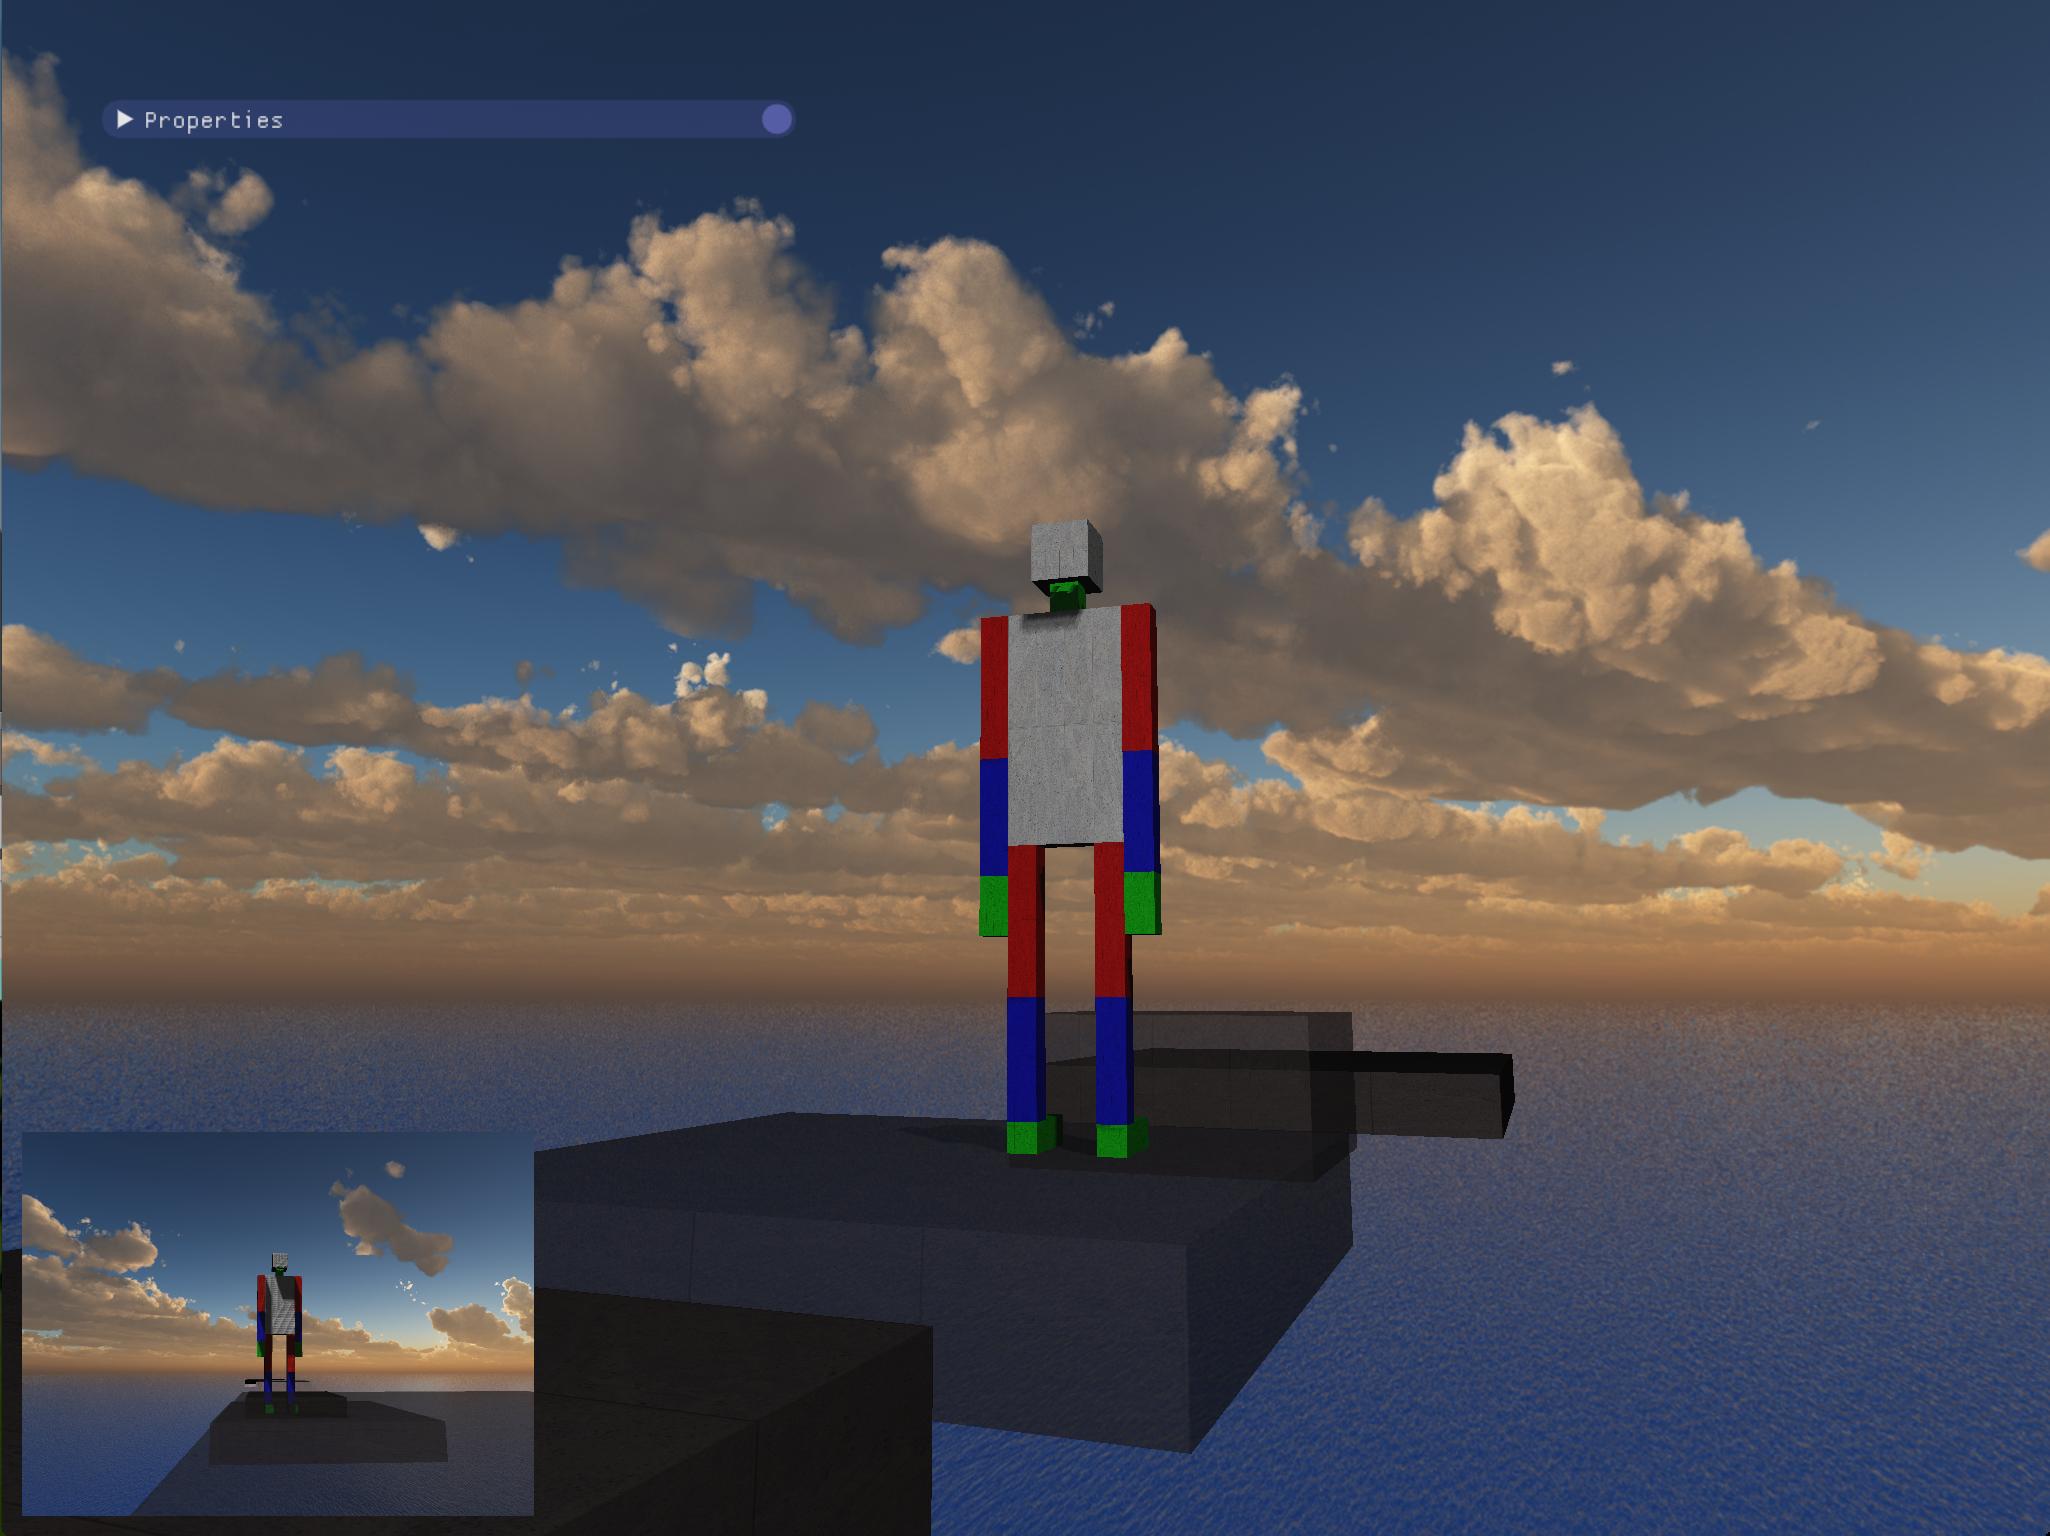
\includegraphics[width=8cm]{transparency}
\centering
\caption{An illustration of transparency within the game.}
\end{figure}

OpenGL is able to render transparent objects correctly. However, if a transparent platform is rendered first and it occludes another platform, which is rendered after, that second platform will not be visible through the first object. The fix for this is to sort all objects with respect to their proximity to the camera and render them in reverse order. This way, the furthest platforms render first and the nearest platforms render last.  This logic is implemented in \verb|A5::renderSceneNormally|.

\subsection{Shadow Mapping}
Since this game has light sources, shadows are also necessary to produce realistic imagery. Since there's no perfect algorithm to implement shadows, most games today rely on shadow approximation techniques to get decent results. The approximation technique I'll be employing in this project is called Shadow Mapping. The general algorithm is described below.

Suppose that we have a singular light source and a world consisting of objects. Then, it's possible to determine whether each point in the world should be in a shadow or not. The scene is visualized in Figure 2.

\begin{figure}[H]
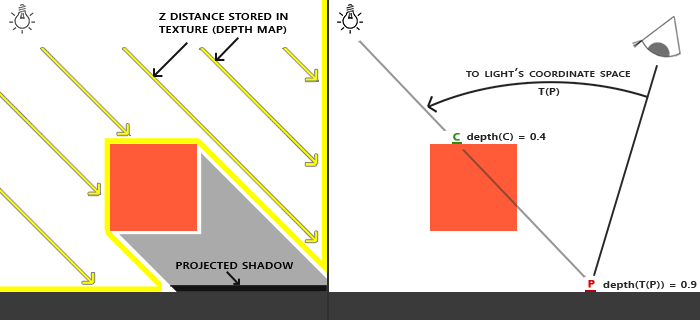
\includegraphics[width=8cm]{shadow_mapping_theory_spaces}
\centering
\caption{An illustration of how to produce shadows using OpenGL's depth buffer\cite{shadow-map-learn-opengl}.}
\end{figure}

The algorithm for shadow mapping is really simple. For each point $P$, we view it from the perspective of the light source. From this perspective, we render the entire scene, using the z-buffer algorithm. This builds a depth buffer, which lets us know for each $(x, y)$, the depth of the closest point to the light source.

After the depth buffer is obtained, we render the scene properly from the perspective of the actual camera. For each fragment, we transform it to the coordinate frame of the light source. Then, before rendering the fragment, we look in the depth buffer at that fragment's transformed $(x, y)$. If the fragment we're trying to render has a depth greater than the depth stored in the depth buffer at point $(x, y)$, then the fragment must be in a shadow. Hence, we render the fragment with darker colour. If the fragment's z value is equal to the z value stored at the depth buffer, then it must be directly illuminated by the light source. In that case, we render it normally.

The actual implementation of the Shadow Map is a bit more nuanced. In implementing the algorithm, one can run into problems such as blocky shadows, Shadow acne, or peter panning. None of these problems were insurmountable, however. The details of the algorithm's implementation are discussed in \cite{shadow-map-learn-opengl}, which is what I used as my primary source to implement the Shadow Mapping in my game.

To implement shadow mapping, I first created another framebuffer explicitly for computing the depth texture. This is accomplished in the \verb|A5::init| method. Once the framebuffer was created, a texture was created and bound as the framebuffer's \verb|GL_DEPTH_ATTACHMENT|. After that, new view and projection matrices were created for the light source, which were used to render the scene from the light's perspective. The matrices were created in \verb|A5::draw| and the depth texture was rendered to in \verb|A5::fillDepthTexture|. This method actually uses a new vertex and fragment shader (\verb|simpleDepthSahder.vsh), and \verb|simpleDepthShader.fsh|, respectively), which are computationally less expensive to run than the main shaders.

With the depth texture filled, it was bound as a uniform before the scene was rendered normally on to the default framebuffer. Within the main fragment shader \verb|Main.fsh|, this texture was sampled in the \verb|ShadowCalculation| function to determine if the current fragment is occluded by some object or not. Normally this calculation would produce either a 1 or a 0, but in \verb|ShadowCalculation|, we sample multiple textels surrounding the current textel to get a gradient between 1 and 0. Ultimately, this produces softer shadows.

\section{Future}
Although the game has a user interface thanks to ImGui, I wanted to create several different screens for the game. For example, a start screen would have been nice to implement. To implement the start screen, I would need some way to render text in OpenGL. This would have added additional complexity to the game, so I did not attempt this goal. In the future, this is one avenue I could explore.

Another aspect of the game that I wanted to explore was adjusting the wind speed factoring in the player's location in the game. One could easily imagine areas of high wind speed and areas of low wind speed. This could add difficulty to the game, and make its levels more interesting.

I also wish that I could have made my puppet more humanoid. In the current implementation of the game, the puppet is derived from my assignment 4 solution. In the future, I could create a puppet using blender and animate that instead. I feel that that change would add a lot of personality to the game.

I would also like to make this game cross platform compatible. Currently, it has only been tested on macOS. It could take some work to get this game to compile for linux, and windows machines. However, doing that work would be worthwhile as not everyone has a Mac.

\chapter{Manual}
The game is fairly simple to compile. The only requirement is that the compilation target be macOS. To compile the game, one must create the \verb|Makefile| using \verb|premake4 gmake|. Then, since this project makes a change to \verb|MeshConsolidator|, the shared code must be compiled. After that, a call to \verb|make| should compile the game. The compiled program should be called \verb|A5|.

There's really one type of input for this program: the levels. Each level is stored in the \verb|Assets| folder. There are three level files in total: \verb|level1.json|, \verb|level2.json|, \verb|level3.json|. Each level is a JSON object with one property: \verb|platforms|. \verb|Platforms| is an array of objects, each of which is deserialized into a \verb|Platform| C++ object in game. The \verb|position|, \verb|size|, and \verb|mass| are fairly self-explanatory. The \verb|ttl| property specifies the platform's lifetime. As long as the player is standing on a platform, it's \verb|ttl| will continually decrease. Once a platform's \verb|ttl| reaches 0, the platform will fall, potentially killing the player and restarting the level. Therefore, the \verb|ttl| property deserializes to the platform's \verb|ttl|, which is a measure of the platform's time to live in seconds. The final property is \verb|updateVFn|. This property describes a sinusoid representing the platform's velocity in the x direction. The sinusoid that \verb|updateVFn| specifies is: $A sin\left(\frac{2\pi}{period}\left(t - k\right)\right) + offset$. Every call to \verb|appLogic|, the velocity of each platform is updated and this function is what calculates the update velocity.

It is also possible to add custom skyboxes into the game. To do so, one must move their skyboxes inside the \verb|Assets/skybox| folder. There should be six skybox images. Suppose the skybox folder name is $X$ and $x = lowercase(X)$ then the image representing the top should be ``x\_up.png''. The image representing the bottom should be named ``x\_dn.png''. The image representing the left should be ``x\_lf.png''. The image representing the right should be ``x\_rt.png''. The image representing the front should be ``x\_ft.png'' and the image representing the back should be named ``x\_bk.png''. Once all the images conform the aforementioned specification, the skymap can be read in by calling \verb|A5::readTextureCubemap(X)| in \verb|A5::init|.

\printbibliography
\newpage
\section{Objectives}
\begin{enumerate}
\item \textbf{Modeling the Scene.} - World objects are rendered on to the screen correctly.
\item \textbf{UI.} - The mouse and keyboard can be used by the player to control the game objects and camera. A GUI also exists for controlling game settings.
\item \textbf{Texture mapping.} - It is evident that texture mapping has been employed at least once.
\item \textbf{Keyframe Animation.} - When the player walks, the puppet plays a walking animation. The current frame is interpolated from its surrounding frames using linear interpolation.
\item \textbf{Static collisions.} - On each stationary platform, the puppet does not fall through the platform and die.
\item \textbf{Dynamic collisions.} - On each moving platform, the puppet does not fall through the platform and die.
\item \textbf{Synchronized sound.} - When the player interacts with the game by moving the puppet, there is audible feedback.
\item \textbf{Physics Engine} - The puppet is subject to gravitational forces (parameter: $g$) and wind force (parameter: $F_w$). The puppet is also subject to static friction when it's standing on a platform. The static friction is a function of the puppet's mass (parameter: $M$) and the platform's normal.
\item \textbf{Transparency} - Transparency will be implemented using the alpha channel. At least one game object is transparent.
\item \textbf{Shadows} - Shadows are implemented using shadow maps.
\end{enumerate}

\textbf{Declaration:}

I have read the statements regarding cheating in the CS488/688 course handouts. I affirm with my signature that I have worked out my own solution to this assignment, and the code I am handing in is my own.

\textbf{Signature:}

\end{document}
